\section{Reti Multimediali}
Le applicazioni multimediali, come lo streaming video (Netflix, YouTube) e la telefonia su Internet (VoIP, Skype, Teams), sono tra le più esigenti in termini di risorse di rete. A differenza di applicazioni "elastiche" come l'email o il web (che funzionano comunque, anche se lentamente), le applicazioni multimediali sono sensibili ai ritardi e alla perdita di dati.

\subsection{Proprietà dei flussi multimediali}
\begin{itemize}
    \item \textbf{Bit Rate Elevato:} Lo streaming video, anche se compresso, richiede un throughput significativamente maggiore rispetto ad altre applicazioni.
    \item \textbf{Compressione:} I flussi audio e video sono quasi sempre compressi (es. H.264/H.265 per il video, MP3/AAC per l'audio) per ridurne il bit rate. Questa compressione può essere \textit{lossy} (con perdita di informazione).
    \item \textbf{Sensibilità al tempo:} Le applicazioni multimediali si dividono in due grandi categorie:
        \begin{itemize}
            \item \textbf{Streaming di contenuti registrati (on-demand):} Come Netflix o YouTube. Non sono sensibili ai ritardi lunghi (possiamo aspettare qualche secondo per l'inizio), ma sono sensibili alle variazioni del throughput.
            \item \textbf{Conversazionali (real-time):} Come VoIP o videoconferenze (Skype). Sono estremamente sensibili ai ritardi end-to-end (idealmente < 150ms, massimo 400ms). Possono però tollerare una piccola perdita di pacchetti.
        \end{itemize}
\end{itemize}

\subsection{Streaming di Video Registrato}
La sfida principale dello streaming video (es. Netflix) su Internet è che la rete IP offre un servizio \textit{best-effort}: il throughput tra server e client può variare ampiamente a causa della congestione.

\subsubsection{Streaming HTTP (DASH)}
Oggi, quasi tutto lo streaming video (incluso YouTube e Netflix) non usa più UDP, ma avviene tramite \textbf{HTTP} su \textbf{TCP}. Questo approccio sfrutta l'affidabilità di TCP e attraversa facilmente i firewall (dato che usa la porta 80/443, sempre aperta).

La soluzione moderna per gestire la variabilità della rete si chiama \textbf{DASH (Dynamic Adaptive Streaming over HTTP)}.
\begin{itemize}
    \item \textbf{Codifica Multipla:} Il server non memorizza un singolo file video, ma \textit{molte versioni} dello stesso video, codificate a diversi bit rate (es. bassa qualità, SD, HD, 4K). Ogni versione è spezzettata in "chunk" (frammenti) di pochi secondi.
    \item \textbf{Manifest File:} Il server fornisce al client un "file manifesto" (manifest file) che elenca tutti i chunk disponibili e i loro bit rate.
    \item \textbf{Logica Adattiva sul Client:} È il \textit{client} (il player) che comanda. Misura la banda disponibile e decide quale chunk richiedere:
        \begin{enumerate}
            \item Se la banda è alta, richiede il prossimo chunk alla qualità 4K.
            \item Se la rete rallenta (congestione), richiede il prossimo chunk alla qualità SD.
        \end{enumerate}
    \item \textbf{Buffering Client:} Il client mantiene un \textbf{buffer di riproduzione} (playout buffer). Cerca di scaricare i chunk più velocemente di quanto li riproduce (es. scarica 10 secondi di video in 2 secondi) per accumulare un "cuscinetto" di dati. Questo buffer assorbe le variazioni di throughput (jitter) della rete, garantendo una riproduzione fluida. Se il buffer si svuota (underflow), la riproduzione si blocca (\textit{stalling}).
\end{itemize}

\begin{center}
    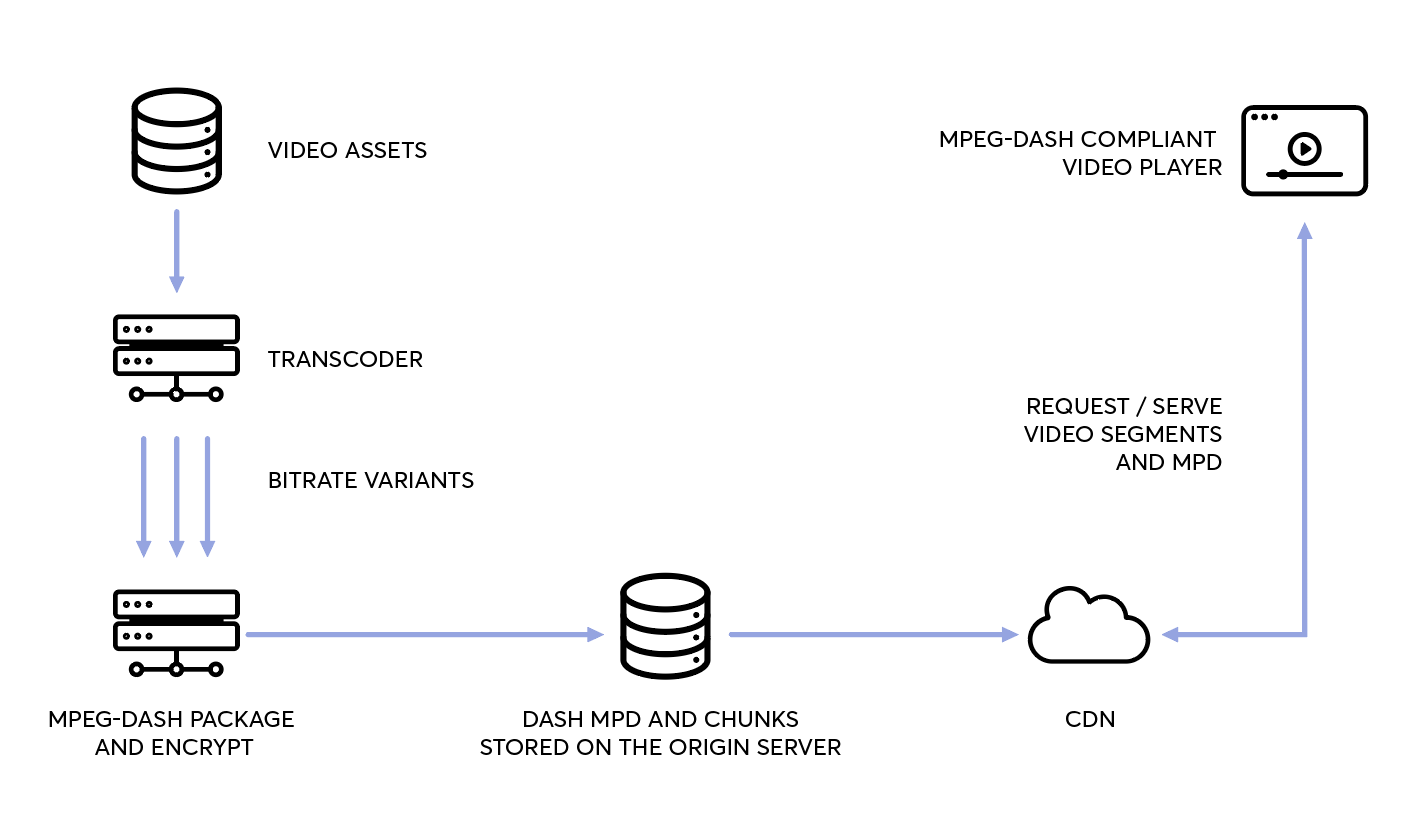
\includegraphics[width=0.7\textwidth]{img/dash_streaming.png}
\end{center}

\subsection{Voice-over-IP (VoIP)}
A differenza dello streaming on-demand, VoIP è conversazionale e non può tollerare grandi ritardi. Per questo, VoIP usa quasi sempre \textbf{UDP}.
Questo introduce due problemi principali:

\subsubsection{Jitter dei Pacchetti}
Il servizio IP best-effort non garantisce solo il ritardo, ma nemmeno che i pacchetti arrivino a intervalli regolari. Un pacchetto può impiegare 20ms e il successivo 80ms. Questa variazione nel ritardo end-to-end è chiamata \textbf{Jitter}.

Per compensare il jitter, il ricevitore VoIP usa un \textbf{buffer di riproduzione (playout buffer)}.
\begin{itemize}
    \item Il ricevitore non riproduce i pacchetti audio appena arrivano.
    \item Li "parcheggia" in un buffer per un breve periodo (es. 20-40ms), per assorbire le variazioni di arrivo.
    \item Quindi li riproduce a intervalli perfettamente costanti, ricostruendo la cadenza della voce originale.
    \item \textbf{Trade-off:} Un buffer grande gestisce meglio il jitter, ma introduce un ritardo artificiale che rende la conversazione innaturale. Un buffer piccolo è reattivo, ma i pacchetti che arrivano troppo tardi (oltre il tempo di riproduzione) vengono \textbf{scartati come se fossero persi}.
\end{itemize}

\subsubsection{Recupero dei Pacchetti Persi}
Dato che VoIP usa UDP, i pacchetti persi non vengono ritrasmessi da TCP. La ritrasmissione sarebbe comunque inutile, perché il pacchetto ritrasmesso arriverebbe troppo tardi per la conversazione. Si usano quindi tecniche di \textbf{Loss Recovery} (Recupero delle Perdite):
\begin{itemize}
    \item \textbf{Forward Error Correction (FEC):} Il mittente invia informazioni ridondanti \textit{prima} che avvenga la perdita. Un metodo comune è inviare, insieme al pacchetto $n$, una versione a bassa qualità (o un XOR) del pacchetto $n-1$. Se il pacchetto $n-1$ si perde, il ricevitore può usare la copia ridondante nel pacchetto $n$ per ricostruirlo. Aumenta il consumo di banda.
    \item \textbf{Interleaving (Interfogliazione):} Il mittente "mescola" i campioni audio prima di inviarli. Ad esempio, un pacchetto contiene i campioni 1, 5, 9, 13 e il pacchetto successivo contiene 2, 6, 10, 14. Se un pacchetto si perde, il ricevitore non avrà un "buco" di dati contigui, ma tante piccole perdite sparse (es. mancano i campioni 5, 6, 7, 8). Queste piccole perdite sono più facili da "nascondere" (es. ripetendo il campione precedente). Introduce un piccolo ritardo aggiuntivo.
\end{itemize}

\subsection{Protocolli per applicazioni in tempo reale}
Per supportare VoIP e streaming, sono stati creati due protocolli a livello applicazione.

\subsubsection{RTP (Real-time Transport Protocol)}
\textbf{RTP} è il protocollo standard per \textit{trasportare} i dati multimediali (audio e video) su Internet.
\begin{itemize}
    \item RTP \textbf{non} è un protocollo di trasporto. Gira \textit{sopra} \textbf{UDP}.
    \item Fornisce servizi che a UDP mancano, ma che sono essenziali per il multimedia.
    \item \textbf{Header RTP:} L'header RTP viene aggiunto al payload (es. campioni audio) prima di inserirlo nel segmento UDP. I suoi campi chiave sono:
        \begin{itemize}
            \item \textbf{Tipo di Payload (Payload Type):} Indica il tipo di codifica audio/video usata (es. G.711, MP3, H.264), permettendo al ricevitore di cambiare decodificatore al volo.
            \item \textbf{Numero di Sequenza (Sequence Number):} Un numero (1, 2, 3...) che permette al ricevitore di rilevare pacchetti persi e riordinare quelli arrivati fuori sequenza.
            \item \textbf{Marcatura Temporale (Timestamp):} Indica l'istante di \textit{campionamento} del primo byte del pacchetto. È fondamentale per il ricevitore per calcolare il jitter e temporizzare correttamente la riproduzione nel buffer.
        \end{itemize}
\end{itemize}
Accanto a RTP, gira \textbf{RTCP} (RTP Control Protocol), che invia periodicamente pacchetti di controllo per monitorare la qualità della sessione (es. statistiche su perdita, jitter, RTT).

\subsubsection{SIP (Session Initiation Protocol)}
Mentre RTP \textit{trasporta} la chiamata, \textbf{SIP} è il protocollo che la \textit{crea}, \textit{gestisce} e \textit{termina}. È il protocollo di \textbf{segnalazione} alla base della maggior parte di VoIP.
\begin{itemize}
    \item \textbf{Basato su testo (come HTTP):} SIP usa messaggi di testo leggibili, come \texttt{INVITE} (per iniziare una chiamata), \texttt{OK}, \texttt{BYE}.
    \item \textbf{Funzionamento (semplificato):}
        \begin{enumerate}
            \item Alice vuole chiamare Bob. Alice invia un messaggio \texttt{INVITE} a un \textbf{SIP Proxy} (un server).
            \item Il server SIP (usando un \textbf{Registrar}) sa a quale indirizzo IP è attualmente registrato Bob (che potrebbe essere a casa o in ufficio).
            \item Il Proxy inoltra l'\texttt{INVITE} a Bob.
            \item Il telefono di Bob squilla e Bob accetta, inviando un \texttt{OK}.
            \item Alice invia un \texttt{ACK}. La chiamata è stabilita.
        \end{enumerate}
    \item \textbf{Separazione Media/Controllo:} SIP stabilisce solo la chiamata. I dati multimediali veri e propri (la voce) fluiscono \textbf{direttamente} tra Alice e Bob usando \textbf{RTP/UDP}, senza passare per il server SIP.
\end{itemize}

\subsection{Supporto di Rete per la Qualità del Servizio (QoS)}
Fino ad ora abbiamo visto come le \textit{applicazioni} cercano di adattarsi alla rete best-effort. Ma cosa può fare la \textit{rete} (l'ISP) per aiutarle?.
L'obiettivo è fornire una \textbf{Qualità del Servizio (QoS)} migliore, differenziando il traffico.

\subsubsection{Differentiated Services (DiffServ)}
Questo è l'approccio alla QoS più diffuso nelle reti degli ISP, perché è scalabile (non richiede ai router di mantenere lo stato per ogni singola chiamata VoIP).

\textbf{Idea Chiave:} Non trattare tutti i pacchetti allo stesso modo. I pacchetti vengono divisi in \textbf{classi}.
\begin{itemize}
    \item \textbf{Marcatura (Marking):} I pacchetti vengono "marcati" (etichettati) quando entrano nella rete dell'ISP (al router di bordo). La marcatura avviene usando un campo nell'header IP chiamato \textbf{DS Field} (Differentiated Services field).
        \begin{itemize}
            \item Esempio: Il traffico VoIP viene marcato come \textbf{EF (Expedited Forwarding)} (alta priorità, basso ritardo).
            \item Il traffico "importante" (es. VPN business) come \textbf{AF (Assured Forwarding)} (banda minima garantita).
            \item Tutto il resto (es. web) come \textbf{BE (Best-Effort)} (nessuna garanzia).
        \end{itemize}
    \item \textbf{Gestione nel Core (PHB):} I router interni (core router) dell'ISP non eseguono logica complessa. Guardano solo il marcatore DS del pacchetto e applicano un \textbf{Per-Hop Behavior (PHB)} (comportamento per-hop).
    \item \textbf{Scheduling nelle Code:} Il PHB viene implementato tramite lo \textbf{scheduling delle code} (discusso nel cap. 4). Ad esempio, si usa l'\textit{accodamento prioritario} (priority queuing): se nella porta di uscita di un router arrivano un pacchetto VoIP (EF) e un pacchetto web (BE), il router trasmetterà \textit{sempre prima} il pacchetto VoIP.
\end{itemize}
In questo modo, il traffico sensibile al ritardo (come VoIP) "salta la fila" all'interno dei router dell'ISP, sperimentando basse perdite e basso jitter, anche quando la rete è congestionata dal traffico best-effort.

\subsubsection{Controllo di Ammissione (Call Admission)}
L'approccio DiffServ migliora le prestazioni, ma non offre garanzie \textit{assolute}. Se 1000 persone provano a fare una chiamata VoIP su un link che ne supporta solo 500, la qualità crollerà per tutti, anche se hanno priorità EF.

Un approccio più rigoroso (ma molto più complesso e quasi mai implementato su Internet pubblica) è il \textbf{Controllo di Ammissione (Call Admission)}:
\begin{itemize}
    \item Prima di iniziare la chiamata (es. con SIP), l'applicazione deve \textit{chiedere il permesso} alla rete, dichiarando di aver bisogno (es.) di 100 kbps.
    \item La rete (tramite un protocollo di segnalazione come RSVP) controlla se ha 100 kbps disponibili lungo \textit{tutto} il percorso.
    \item Solo se la banda c'è, la chiamata viene "ammessa" e le risorse vengono \textit{riservate}. Altrimenti, la chiamata viene rifiutata (segnale di occupato).
\end{itemize}
